% =============================================================================
%  Diplomado en Data Science Aplicada con Python para la Toma de Decisiones
%  Clase 33: Introduccion a NLP - de representar texto a entender el contexto
%  Arca Continental Ecuador | UDLA
% =============================================================================
\documentclass[aspectratio=169, 11pt]{beamer}

\usepackage[T1]{fontenc}
\usepackage[utf8]{inputenc}
\usepackage[spanish,es-noshorthands]{babel}
\usepackage{FiraSans}
\usepackage{FiraMono}
\renewcommand{\familydefault}{\sfdefault}
\usepackage{graphicx}
\usepackage{tikz}
\usetikzlibrary{arrows.meta, positioning, shapes.geometric, shapes.misc,
  calc, fit, decorations.pathreplacing, backgrounds, matrix, chains}
\usepackage{fontawesome5}
\usepackage{minted}
\usepackage{tcolorbox}
\tcbuselibrary{minted, skins, breakable}
\usepackage{booktabs}
\usepackage{colortbl}
\usepackage{multicol}
\usepackage{hyperref}
\usepackage{calc}
\usepackage{amsmath}

\definecolor{arcaRed}{HTML}{C82B40}
\definecolor{arcaDark}{HTML}{6B1525}
\definecolor{udlaCrimson}{HTML}{A31545}
\definecolor{arcaGray}{HTML}{F5F5F5}
\definecolor{arcaLightGray}{HTML}{EBEBEB}
\definecolor{textDark}{HTML}{2D2D2D}
\definecolor{textMuted}{HTML}{6B7280}
\definecolor{codeGreen}{HTML}{16A34A}
\definecolor{codeBlue}{HTML}{2563EB}
\definecolor{codeOrange}{HTML}{EA580C}
\definecolor{codePurple}{HTML}{7C3AED}

\usetheme{default}
\usecolortheme{default}
\setbeamertemplate{navigation symbols}{}
\setbeamertemplate{footline}{}
\setbeamertemplate{headline}{}
\setbeamercolor{normal text}{fg=textDark}
\setbeamercolor{frametitle}{fg=arcaRed, bg=white}
\setbeamercolor{title}{fg=white}
\setbeamercolor{subtitle}{fg=white!85}
\setbeamercolor{author}{fg=white!80}
\setbeamercolor{date}{fg=white!70}
\setbeamercolor{item}{fg=arcaRed}
\setbeamercolor{subitem}{fg=arcaDark}
\setbeamercolor{block title}{fg=white, bg=arcaRed}
\setbeamercolor{block body}{fg=textDark, bg=arcaGray}
\setbeamercolor{section in toc}{fg=arcaDark}
\setbeamerfont{frametitle}{size=\Large, series=\bfseries}
\setbeamerfont{title}{size=\huge, series=\bfseries}
\setbeamerfont{subtitle}{size=\large}
\setbeamerfont{author}{size=\normalsize}
\setbeamerfont{date}{size=\small}
\setbeamerfont{block title}{size=\normalsize, series=\bfseries}
\setbeamerfont{footnote}{size=\tiny}
\setbeamertemplate{itemize item}{\scriptsize\raise1.5pt\hbox{\color{arcaRed}$\blacktriangleright$}}
\setbeamertemplate{itemize subitem}{\scriptsize\raise1pt\hbox{\color{arcaDark}$\bullet$}}
\setbeamertemplate{enumerate items}[default]
\setbeamercolor{enumerate item}{fg=arcaRed}

\setbeamertemplate{headline}{%
  \begin{tikzpicture}[remember picture, overlay]
    \fill[arcaDark] (current page.north west) rectangle
      ([yshift=-0.7cm]current page.north east);
    \node[anchor=west, inner sep=0pt] at
      ([xshift=0.6cm, yshift=-0.35cm]current page.north west)
      {
\includegraphics[height=0.45cm]{../logo_udla_white.png}};
    \node[anchor=east, inner sep=0pt] at
      ([xshift=-0.6cm, yshift=-0.35cm]current page.north east)
      {
\includegraphics[height=0.45cm]{../ArcaContinental_white.png}};
  \end{tikzpicture}%
  \vspace{0.7cm}%
}

\setbeamertemplate{footline}{%
  \begin{tikzpicture}[remember picture, overlay]
    \node[anchor=south east, font=\scriptsize\bfseries\color{arcaRed}] at
      ([xshift=-0.5cm, yshift=0.15cm]current page.south east)
      {\insertframenumber};
  \end{tikzpicture}%
  \vspace{0.3cm}%
}

\setbeamertemplate{frametitle}{%
  \vspace{0.25cm}%
  \usebeamerfont{frametitle}\usebeamercolor[fg]{frametitle}\insertframetitle%
  \par\vspace{2pt}%
  \begin{tikzpicture}
    \fill[arcaRed] (0,0) rectangle (3cm, 1.5pt);
    \fill[arcaLightGray] (3cm,0) rectangle (\textwidth, 0.5pt);
  \end{tikzpicture}%
  \vspace{0.1cm}%
}

\newtcblisting{pyblock}[1][]{%
  listing engine=minted, minted language=python, minted style=friendly,
  minted options={fontsize=\small, linenos=false, breaklines=true, python3=true},
  colback=arcaGray, colframe=arcaRed, left=4pt, right=4pt, top=4pt, bottom=4pt,
  boxrule=0pt, leftrule=3pt, arc=2pt, listing only, #1}

\newcommand{\sectionframe}[2]{%
  \begingroup
  \setbeamertemplate{headline}{}%
  \setbeamertemplate{footline}{}%
  \begin{frame}[plain, noframenumbering]
    \begin{tikzpicture}[remember picture, overlay]
      \fill[arcaRed] (current page.south west) rectangle (current page.north east);
      \node[anchor=center, text=white, font=\Huge\bfseries, text width=12cm,
            align=center] at ([yshift=0.5cm]current page.center) {#1};
      \node[anchor=center, text=white!80, font=\large, text width=10cm,
            align=center] at ([yshift=-0.8cm]current page.center) {#2};
    \end{tikzpicture}
  \end{frame}
  \endgroup
}

% --- estilos TikZ reutilizables ---
\tikzset{
  conceptbox/.style={draw, rounded corners=3pt, thick, align=center, font=\footnotesize, inner sep=5pt},
  doccard/.style={draw=textMuted, fill=white, rounded corners=2pt, minimum width=2cm, minimum height=1.5cm},
  flowarr/.style={-{Stealth[length=2.2mm]}, arcaRed, thick},
}

\title{Diplomado en Data Science Aplicada\\con Python para la Toma de Decisiones}
\subtitle{Clase 33: Introduccion a NLP --- de representar texto a entender el contexto}
\author{Carlos Enrique Mosquera Trujillo}
\date{29 de Mayo, 2026}

\begin{document}

% ===================== PORTADA =====================
{
\setbeamertemplate{headline}{}
\setbeamertemplate{footline}{}
\begin{frame}[plain, noframenumbering]
  \begin{tikzpicture}[remember picture, overlay]
    \fill[arcaDark] (current page.south west) rectangle (current page.north east);
    \fill[arcaRed] ([yshift=-3.5cm]current page.north west) rectangle
      ([yshift=-4.2cm]current page.north east);
    \node[anchor=west, inner sep=0pt] at
      ([xshift=1cm, yshift=-1.5cm]current page.north west)
      {
\includegraphics[height=1cm]{../logo_udla_white.png}};
    \node[anchor=east, inner sep=0pt] at
      ([xshift=-1cm, yshift=-1.5cm]current page.north east)
      {
\includegraphics[height=1cm]{../ArcaContinental_white.png}};
  \end{tikzpicture}
  \vspace{2.5cm}
  \begin{center}
    {\usebeamerfont{title}\usebeamercolor[fg]{title}\inserttitle\par}
    \vspace{0.4cm}
    {\usebeamerfont{subtitle}\usebeamercolor[fg]{subtitle}\insertsubtitle\par}
    \vspace{0.6cm}
    {\usebeamerfont{author}\usebeamercolor[fg]{author}\insertauthor\par}
    \vspace{0.15cm}
    {\usebeamerfont{date}\usebeamercolor[fg]{date}\insertdate\par}
  \end{center}
\end{frame}
}

% ===================== HERO =====================
{
\setbeamertemplate{headline}{}
\setbeamertemplate{footline}{}
\begin{frame}[plain, noframenumbering]
  \begin{center}
\includegraphics[width=\paperwidth]{fig_hero.png}\end{center}
\end{frame}
}

% ===================== BLOQUE 0 =====================
\sectionframe{Bloque 0}{El problema:\\enseñarle a la máquina qué significa el texto}

\begin{frame}[shrink]{Dónde estamos en el diplomado}
  \vspace{4pt}
  {\footnotesize\color{arcaDark}Los tipos de dato que ya modelamos:\par}
  \vspace{6pt}
  \begin{itemize}\setlength{\itemsep}{4pt}\footnotesize
    \item \textbf{Tablas} (Módulo 4): filas y columnas numéricas $\rightarrow$ clasificación, clustering.
    \item \textbf{Imágenes} (clase 28--29): una matriz de píxeles $\rightarrow$ CNN, autoencoders.
    \item \textbf{Series temporales} (clase 31--32): una secuencia de valores $\rightarrow$ Prophet, LSTM.
  \end{itemize}
  \vspace{8pt}
  \begin{tcolorbox}[colback=arcaRed!8, colframe=arcaRed, leftrule=3pt, boxrule=0pt, sharp corners, left=8pt, right=8pt, top=4pt, bottom=4pt]
    {\small\color{arcaDark}\bfseries
    Hoy entra el \textbf{texto}. La pregunta de toda la clase: ¿cómo convertimos texto en números
    que capturen su \textbf{significado}, para poder clasificarlo y buscarlo?}
  \end{tcolorbox}
\end{frame}

\begin{frame}[shrink]{Ponte en el lugar de la máquina}
  \begin{center}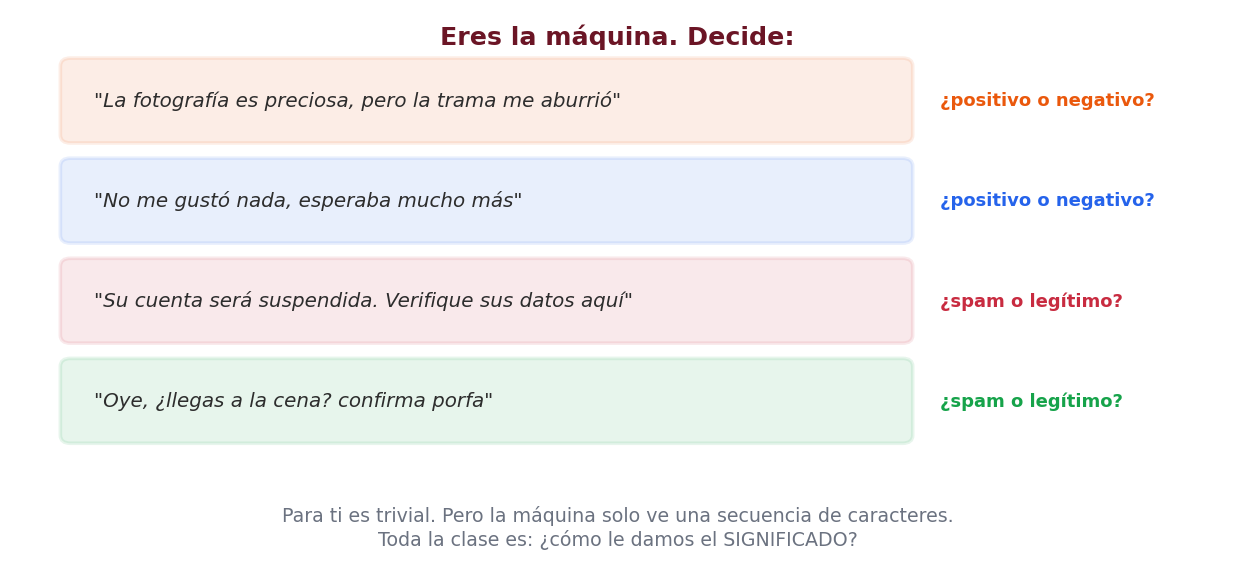
\includegraphics[width=0.97\textwidth]{fig_problema_descubrimiento.png}\end{center}
  \vspace{2pt}
  \begin{tcolorbox}[colback=arcaGray, colframe=arcaRed, leftrule=3pt, boxrule=0pt, sharp corners, left=8pt, right=8pt, top=4pt, bottom=4pt]
    {\footnotesize\color{arcaDark}
    \textbf{Pregunta para el aula:} ¿qué información necesitaría la máquina para acertar la 2ª y la
    3ª frase? Guarda tu respuesta: la iremos resolviendo a lo largo de la clase.}
  \end{tcolorbox}
\end{frame}

\begin{frame}[shrink]{Las 4 familias de problemas de NLP}
  \begin{center}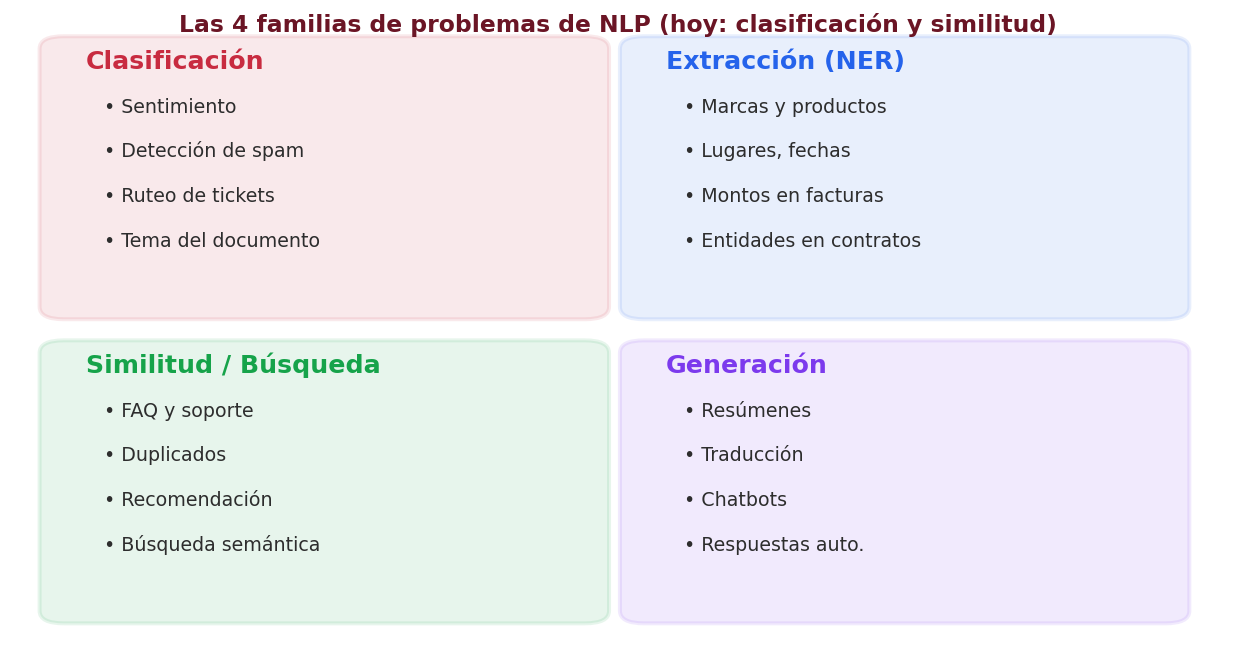
\includegraphics[width=0.97\textwidth]{fig_que_es_nlp.png}\end{center}
  \vspace{2pt}
  {\footnotesize\color{arcaDark}
  \textbf{NLP} = técnicas para que una máquina procese lenguaje humano y tome decisiones. Hoy:
  clasificación (sentimiento, spam) y similitud (búsqueda semántica).}
\end{frame}

\begin{frame}[shrink]{El recorrido de hoy --- 4 formas de representar texto}
  \vspace{6pt}
  \begin{center}
  \begin{tikzpicture}[node distance=1.0cm]
    \node[conceptbox, draw=codeBlue, fill=codeBlue!8, minimum height=1.5cm, text width=2.3cm] (a)
      {\textbf{1. Conteo}\\[2pt]{\scriptsize Bag-of-Words}\\{\scriptsize cuántas veces}};
    \node[conceptbox, draw=codeOrange, fill=codeOrange!8, minimum height=1.5cm, text width=2.3cm, right=of a] (b)
      {\textbf{2. Pesado}\\[2pt]{\scriptsize TF-IDF}\\{\scriptsize cuáles importan}};
    \node[conceptbox, draw=codeGreen, fill=codeGreen!8, minimum height=1.5cm, text width=2.3cm, right=of b] (c)
      {\textbf{3. Significado}\\[2pt]{\scriptsize Embeddings}\\{\scriptsize qué quiere decir}};
    \node[conceptbox, draw=codePurple, fill=codePurple!8, minimum height=1.5cm, text width=2.3cm, right=of c] (d)
      {\textbf{4. Contexto}\\[2pt]{\scriptsize Atención}\\{\scriptsize según la frase}};
    \draw[flowarr] (a)--(b); \draw[flowarr] (b)--(c); \draw[flowarr] (c)--(d);
  \end{tikzpicture}
  \end{center}
  \vspace{6pt}
  \begin{tcolorbox}[colback=arcaRed!8, colframe=arcaRed, leftrule=3pt, boxrule=0pt, sharp corners, left=8pt, right=8pt, top=4pt, bottom=4pt]
    {\footnotesize\color{arcaDark}
    Empezamos por lo más simple (contar) y avanzamos cuando ese enfoque se queda corto. Cada técnica
    captura algo que la anterior no podía.}
  \end{tcolorbox}
\end{frame}

% ===================== BLOQUE 1 =====================
\sectionframe{Bloque 1}{De texto a números}

\begin{frame}[shrink]{La cadena: del texto a un vector de números}
  \vspace{8pt}
  \begin{center}
  \begin{tikzpicture}[node distance=0.75cm]
    \node[conceptbox, draw=arcaDark, fill=arcaDark!6, text width=1.9cm, minimum height=1.5cm] (t)
      {\textbf{TEXTO}\\[2pt]{\scriptsize\ttfamily "No me gustó"}};
    \node[conceptbox, draw=codePurple, fill=codePurple!8, text width=1.9cm, minimum height=1.5cm, right=of t] (c)
      {\textbf{CARACTERES}\\[2pt]{\scriptsize\ttfamily N\,o\,\,m\,e ...}};
    \node[conceptbox, draw=codeBlue, fill=codeBlue!8, text width=1.9cm, minimum height=1.5cm, right=of c] (k)
      {\textbf{TOKENS}\\[2pt]{\scriptsize\ttfamily [no][me]\\{}[gusto]}};
    \node[conceptbox, draw=codeOrange, fill=codeOrange!8, text width=1.9cm, minimum height=1.5cm, right=of k] (v)
      {\textbf{VOCABULARIO}\\[2pt]{\scriptsize\ttfamily no$\to$7\\gusto$\to$42}};
    \node[conceptbox, draw=codeGreen, fill=codeGreen!8, text width=1.9cm, minimum height=1.5cm, right=of v] (x)
      {\textbf{VECTOR}\\[2pt]{\scriptsize\ttfamily [7,3,42]}};
    \draw[flowarr] (t)--(c); \draw[flowarr] (c)--(k); \draw[flowarr] (k)--(v); \draw[flowarr] (v)--(x);
  \end{tikzpicture}
  \end{center}
  \vspace{6pt}
  {\footnotesize\color{arcaDark}
  Cada flecha es una \textbf{decisión de diseño}. La más importante: ¿el ``átomo'' es el carácter,
  la palabra o el ``subword''? Hoy trabajamos con \textbf{palabras}.}
\end{frame}

\begin{frame}[shrink]{¿Qué es Unicode?}
  \begin{tcolorbox}[colback=arcaGray, colframe=arcaRed, leftrule=3pt, boxrule=0pt, sharp corners, left=8pt, right=8pt, top=6pt, bottom=6pt]
    {\small\color{arcaDark}
    \textbf{Unicode} es un \textbf{estándar universal} que le asigna a cada carácter de cualquier
    idioma --- letras, acentos, signos, incluso emojis --- un \textbf{número único} llamado
    \emph{code point}. Antes de Unicode, cada sistema usaba su propia tabla y los textos se
    corrompían al pasar de una computadora a otra.}
  \end{tcolorbox}
  \vspace{10pt}
  \begin{center}
  \begin{tikzpicture}[every node/.style={font=\normalsize}]
    \node[font=\footnotesize\ttfamily\color{textDark}] at (-2.2,0) {"café" =};
    \foreach \i/\c/\n in {0/c/99, 1/a/97, 2/f/102, 3/{é}/233}{
      \node[draw=codeBlue, fill=codeBlue!8, rounded corners, minimum size=1cm] (b\i) at (\i*1.5,0) {\c};
      \node[font=\scriptsize\ttfamily, below=2pt of b\i] {\n};
    }
  \end{tikzpicture}
  \end{center}
  \vspace{8pt}
  {\footnotesize\color{arcaDark}
  La máquina nunca ve ``letras'': ve esta \textbf{secuencia de enteros}. Cada carácter $\rightarrow$ un número.}
\end{frame}

\begin{frame}[shrink]{Cómo se codifican varias palabras}
  \begin{center}{\small\ttfamily
  \renewcommand{\arraystretch}{1.4}
  \begin{tabular}{l@{\quad$\rightarrow$\quad}l}
    "hola"  & [104, 111, 108, 97]\\
    "café"  & [99, 97, 102, 233]\\
    "niño"  & [110, 105, 241, 111]\\
    "Sí!"   & [83, 237, 33]\\
  \end{tabular}}
  \end{center}
  \vspace{4pt}
  {\footnotesize\color{arcaDark}
  ``ñ'' es el 241, ``é'' el 233, ``í'' el 237; hasta la carita sonriente tiene su número (el 128578).}
  \vspace{6pt}
  \begin{tcolorbox}[colback=arcaRed!8, colframe=arcaRed, leftrule=3pt, boxrule=0pt, sharp corners, left=8pt, right=8pt, top=4pt, bottom=4pt]
    {\footnotesize\color{arcaDark}
    \textbf{Una trampa:} ``café'' puede ocupar \textbf{4 o 5} code points. Si el acento va pegado
    (``é'' $=233$) son 4; si va aparte (``e'' $+$ ``\,´\,'' $=101+769$) son 5. Se ven igual pero son
    distintos $\rightarrow$ por eso el primer paso siempre es \textbf{normalizar}.}
  \end{tcolorbox}
\end{frame}

\begin{frame}[fragile, shrink]{Tokenizar y normalizar --- en código}
  \begin{pyblock}
import re, unicodedata

def tokenizar(texto):
    texto = texto.lower()                       # minúsculas
    texto = "".join(c for c in unicodedata.normalize("NFD", texto)
                    if unicodedata.category(c) != "Mn")   # quita acentos
    return re.findall(r"[a-zñ]+", texto)        # solo palabras

tokenizar("¡No me GUSTÓ nada!")   # -> ['no', 'me', 'gusto', 'nada']
  \end{pyblock}
  \vspace{2pt}
  {\footnotesize\color{arcaDark}
  \textbf{Tokenizar} = partir el texto en unidades (tokens). \textbf{Normalizar} = unificar variantes
  (mayúsculas, acentos, signos) para que ``GUSTÓ'' y ``gusto'' sean el mismo token.}
\end{frame}

% ===================== BLOQUE 2 =====================
\sectionframe{Bloque 2}{Representar texto contando palabras\\(Bag-of-Words)}

\begin{frame}[shrink]{¿Qué es un corpus?}
  \begin{columns}[c]
    \begin{column}{0.46\textwidth}
      \begin{center}
      \begin{tikzpicture}
        \node[draw=codePurple, very thick, rounded corners, minimum width=5cm, minimum height=3.3cm] (box) {};
        \node[anchor=south, font=\bfseries\color{codePurple}] at (box.north) {CORPUS};
        \node[doccard] at (-1.3,0.55) {};
        \node[doccard] at (1.3,0.55) {};
        \node[doccard] at (-1.3,-0.95) {};
        \node[doccard] at (1.3,-0.95) {};
        \foreach \x/\y in {-1.3/0.55, 1.3/0.55, -1.3/-0.95, 1.3/-0.95}{
          \foreach \dy in {0.45,0.2,-0.05,-0.3}{
            \draw[textMuted!60, line width=1pt] (\x-0.7,\y+\dy) -- (\x+0.7,\y+\dy);}}
      \end{tikzpicture}
      \end{center}
    \end{column}
    \begin{column}{0.5\textwidth}
      {\footnotesize\color{arcaDark}
      Un \textbf{corpus} es la \textbf{colección completa de documentos} con la que trabajamos.\par
      \vspace{8pt}
      Un ``documento'' puede ser una reseña, un SMS, un ticket de soporte, una respuesta de encuesta...\par
      \vspace{8pt}
      \textbf{Ejemplos en Arca:} las 2.600 reseñas de hoy; o todos los comentarios de clientes del
      mes; o todos los tickets de un call center.}
    \end{column}
  \end{columns}
\end{frame}

\begin{frame}[shrink]{¿Qué es el vocabulario?}
  \begin{center}
  \begin{tikzpicture}[node distance=1.4cm]
    \node[conceptbox, draw=textMuted, fill=arcaGray, text width=4.5cm, align=left] (docs)
      {\scriptsize D1: ``gratis gana premio gratis''\\ D2: ``hola la reunión es hoy''};
    \node[conceptbox, draw=codeOrange, fill=codeOrange!8, text width=4.2cm, align=left, right=2.2cm of docs] (voc)
      {\scriptsize\ttfamily gratis$\to$0\quad gana$\to$1\\ premio$\to$2\quad hola$\to$3\\ la$\to$4\quad reunión$\to$5\\ es$\to$6\quad hoy$\to$7};
    \draw[flowarr] (docs) -- node[above, font=\scriptsize\color{textMuted}]{palabras únicas} (voc);
  \end{tikzpicture}
  \end{center}
  \vspace{6pt}
  {\footnotesize\color{arcaDark}
  El \textbf{vocabulario} es el conjunto de \textbf{palabras distintas} del corpus. A cada palabra le
  damos un \textbf{índice} (un número de columna). Su tamaño define cuántas columnas tendrá cada vector
  --- en un corpus real, decenas de miles.}
\end{frame}

\begin{frame}[shrink]{¿Qué es Bag-of-Words (``bolsa de palabras'')?}
  \begin{center}
  \begin{tikzpicture}[node distance=1.1cm]
    \node[conceptbox, draw=textMuted, fill=arcaGray, text width=3.4cm] (d)
      {\scriptsize\ttfamily "gratis gana premio gratis"};
    \node[draw=codeBlue, very thick, rounded corners, fill=codeBlue!6, minimum width=3cm, minimum height=1.8cm, right=of d] (bag)
      {\footnotesize\color{codeBlue}\textbf{bolsa}};
    \node[conceptbox, draw=codeBlue, fill=white, text width=2.6cm, align=left, right=of bag] (cnt)
      {\scriptsize\ttfamily gratis: 2\\ gana: 1\\ premio: 1};
    \draw[flowarr] (d)--(bag); \draw[flowarr] (bag)--(cnt);
  \end{tikzpicture}
  \end{center}
  \vspace{4pt}
  {\footnotesize\color{arcaDark}
  Echo todas las palabras del documento en una ``bolsa'': conservo \textbf{qué} palabras hay y
  \textbf{cuántas} veces, pero \textbf{tiro el orden}.}
  \vspace{4pt}
  \begin{tcolorbox}[colback=codeOrange!8, colframe=codeOrange, leftrule=3pt, boxrule=0pt, sharp corners, left=8pt, right=8pt, top=3pt, bottom=3pt]
    {\footnotesize\color{arcaDark}
    Por eso ``el perro muerde al hombre'' y ``el hombre muerde al perro'' producen \textbf{la misma
    bolsa}. Esa pérdida del orden la pagaremos más tarde.}
  \end{tcolorbox}
\end{frame}

\begin{frame}[shrink]{De las bolsas a una matriz: el ``puente'' a los números}
  \vspace{4pt}
  \begin{center}
  {\footnotesize\renewcommand{\arraystretch}{1.3}
  \begin{tabular}{r|cccccc}
     & \cellcolor{arcaGray}gratis & \cellcolor{arcaGray}gana & \cellcolor{arcaGray}premio & \cellcolor{arcaGray}hola & \cellcolor{arcaGray}reunión & \cellcolor{arcaGray}hoy \\\hline
    \cellcolor{arcaGray}\textbf{D1} & \cellcolor{codeBlue!35}2 & \cellcolor{codeBlue!20}1 & \cellcolor{codeBlue!20}1 & 0 & 0 & 0 \\
    \cellcolor{arcaGray}\textbf{D2} & 0 & 0 & 0 & \cellcolor{codeBlue!20}1 & \cellcolor{codeBlue!20}1 & \cellcolor{codeBlue!20}1 \\
  \end{tabular}}\\[4pt]
  {\scriptsize\color{codeGreen}\textbf{cada FILA es el vector de un documento}}
  \end{center}
  \vspace{4pt}
  \begin{columns}[t]
    \begin{column}{0.5\textwidth}
      {\footnotesize\color{arcaDark}\textbf{El ``puente'':} cada documento se vuelve una fila $=$ un
      vector numérico de largo fijo. Ahora \textbf{cualquier clasificador} (la Regresión Logística del
      Módulo 4) puede comerlo.}
    \end{column}
    \begin{column}{0.5\textwidth}
      {\footnotesize\color{arcaDark}\textbf{¿Por qué ``dispersa''?} Cada documento usa solo un puñado
      de las decenas de miles de palabras del vocabulario $\rightarrow$ casi todas las celdas son
      \textbf{cero}. La matriz es enorme y casi vacía.}
    \end{column}
  \end{columns}
\end{frame}

% ===================== BLOQUE 3 =====================
\sectionframe{Bloque 3}{No todas las palabras valen igual\\(Zipf, stopwords, TF-IDF)}

\begin{frame}[shrink]{El problema del conteo crudo}
  \begin{tcolorbox}[colback=arcaRed!8, colframe=arcaRed, leftrule=3pt, boxrule=0pt, sharp corners, left=8pt, right=8pt, top=5pt, bottom=5pt]
    {\small\color{arcaDark}
    En el conteo, las palabras que más ``puntúan'' son ``de'', ``la'', ``que''... porque son las que
    más se repiten. Pero esas \textbf{no distinguen} una reseña buena de una mala: están en todas.}
  \end{tcolorbox}
  \vspace{6pt}
  {\footnotesize\color{arcaDark}
  Necesitamos darle \textbf{más peso a las palabras informativas} y menos a las comunes. Para
  entender por qué, primero hay que ver un patrón universal del lenguaje: la \textbf{ley de Zipf}.}
\end{frame}

\begin{frame}[shrink]{¿Qué es la ley de Zipf?}
  \begin{columns}[c]
    \begin{column}{0.5\textwidth}
      \begin{center}
      \begin{tikzpicture}[every node/.style={font=\scriptsize}]
        \foreach \i/\h/\w in {1/2.6/de, 2/1.3/la, 3/0.87/que, 4/0.65/y, 5/0.52/en}{
          \fill[codeBlue!70] (\i*0.9,0) rectangle (\i*0.9+0.55,\h);
          \node at (\i*0.9+0.27,-0.22) {\w};
          \node[font=\tiny\color{textMuted}] at (\i*0.9+0.27,\h+0.18) {$\sim\!\frac{1}{\i}$};}
        \draw[->] (0.6,0)--(5.6,0); \draw[->] (0.7,-0.02)--(0.7,3);
        \node[rotate=90, font=\tiny\color{textMuted}] at (0.45,1.4) {frecuencia};
        \node[font=\tiny\color{textMuted}] at (3,-0.55) {palabras ordenadas por rango};
      \end{tikzpicture}
      \end{center}
    \end{column}
    \begin{column}{0.5\textwidth}
      {\footnotesize\color{arcaDark}
      \textbf{Rango} = la posición de una palabra cuando las ordenas de la \textbf{más} a la
      \textbf{menos} frecuente. La más frecuente (``de'') tiene rango 1; la siguiente (``la''),
      rango 2; y así.\par
      \vspace{5pt}
      Zipf observó que la \textbf{frecuencia es $\approx$ inversa al rango}: la palabra de rango 1
      aparece $\sim$2$\times$ la de rango 2, $\sim$3$\times$ la de rango 3, $\sim$10$\times$ la de
      rango 10.\par
      \vspace{5pt}
      Es una regularidad \textbf{universal} (cualquier idioma): unas pocas palabras acaparan casi
      todo el texto; la mayoría aparece poquísimo.}
    \end{column}
  \end{columns}
\end{frame}

\begin{frame}[shrink]{Zipf en nuestro corpus (datos reales)}
  \begin{center}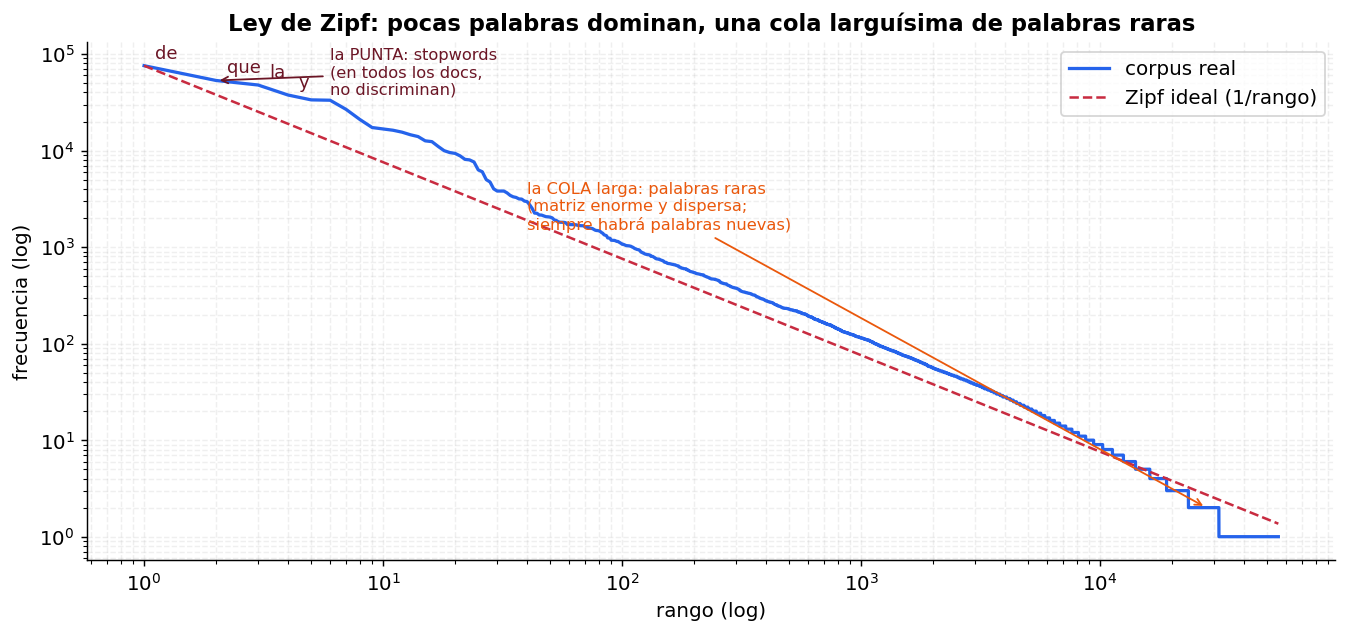
\includegraphics[width=0.8\textwidth]{fig_zipf.png}\end{center}
  \vspace{2pt}
  {\footnotesize\color{arcaDark}
  En escala log-log (cada paso $\times$10), la relación ``frecuencia $\approx 1/$rango'' se ve como
  una \textbf{línea recta}: esa es la ``firma'' de Zipf. Nuestro corpus de reseñas la cumple.}
\end{frame}

\begin{frame}[shrink]{Qué consecuencias tiene Zipf (con calma)}
  \vspace{4pt}
  \begin{enumerate}\setlength{\itemsep}{7pt}\footnotesize
    \item[\textbf{1.}] \textbf{Hay stopwords.} Las palabras del tope (``de'', ``la'', ``que'') aparecen
      en \emph{casi todos} los documentos. Como están en todos, no ayudan a distinguir una reseña
      buena de una mala $\rightarrow$ aportan poca señal. A esas palabras tan comunes y vacías de
      contenido las llamamos \textbf{stopwords}.
    \item[\textbf{2.}] \textbf{El conteo crudo engaña.} Como esas pocas palabras dominan los conteos,
      un modelo que use conteo crudo se fijaría sobre todo en ``de/la/que''. Hay que \textbf{bajarles
      el peso} y subírselo a las palabras raras pero informativas. Ese reajuste es exactamente lo que
      hace \textbf{TF-IDF} (siguiente slide).
    \item[\textbf{3.}] \textbf{La cola larga trae dos cosas.} La inmensa mayoría de palabras aparece
      una o dos veces. Eso significa: (a) el vocabulario es enorme pero cada documento usa poquísimas
      $\rightarrow$ la \textbf{matriz es casi toda ceros} (dispersa); y (b) siempre llegará una palabra
      \textbf{nueva} que el modelo no vio al entrenar.
  \end{enumerate}
\end{frame}

\begin{frame}[shrink]{¿Qué son las stopwords?}
  \begin{center}
  \begin{tikzpicture}[node distance=2pt, every node/.style={font=\small}]
    \node[draw=textMuted, fill=textMuted!12, rounded corners, inner sep=3pt] (a) {la};
    \node[draw=codeGreen, fill=codeGreen!12, rounded corners, inner sep=3pt, right=of a] (b) {película};
    \node[draw=textMuted, fill=textMuted!12, rounded corners, inner sep=3pt, right=of b] (c) {es};
    \node[draw=textMuted, fill=textMuted!12, rounded corners, inner sep=3pt, right=of c] (d) {una};
    \node[draw=codeGreen, fill=codeGreen!12, rounded corners, inner sep=3pt, right=of d] (e) {obra};
    \node[draw=codeGreen, fill=codeGreen!12, rounded corners, inner sep=3pt, right=of e] (f) {maestra};
  \end{tikzpicture}
  \end{center}
  \vspace{2pt}
  {\footnotesize\color{arcaDark}
  Las \textbf{stopwords} (en gris) son palabras muy frecuentes y poco informativas: artículos,
  preposiciones, conjunciones (``la, es, una, de, y''). Las palabras de \textbf{contenido} (en verde)
  son las que dicen de qué trata el texto.}
  \vspace{4pt}
  \begin{tcolorbox}[colback=arcaGray, colframe=arcaRed, leftrule=3pt, boxrule=0pt, sharp corners, left=8pt, right=8pt, top=4pt, bottom=4pt]
    {\footnotesize\color{arcaDark}
    \textbf{¿Se quitan?} En los modelos clásicos (como el de hoy) \textbf{sí}, normalmente se eliminan:
    reducen ruido y achican la matriz. \textbf{Pero hoy en día, en los modelos modernos
    (transformers), NO se quitan} --- para ellos el contexto importa, y ``no'' (una stopword) puede
    invertir toda una frase.}
  \end{tcolorbox}
\end{frame}

\begin{frame}[shrink]{¿Qué es TF-IDF? Pesar una palabra por su rareza}
  \vspace{2pt}
  {\footnotesize\color{arcaDark}\textbf{``Rareza'' = en cuántos documentos aparece la palabra} (su
  \emph{document frequency}, df). Una palabra rara aparece en pocos documentos $\rightarrow$ es muy
  informativa cuando aparece.\par}
  \vspace{4pt}
  \begin{center}
  \begin{tikzpicture}[every node/.style={font=\scriptsize}]
    \node[align=left, text width=4.0cm] (docs) {Corpus de 3 documentos:\\ D1: ``la película es buena''\\ D2: ``la película es mala''\\ D3: ``la película es lenta''};
    \node[align=left, right=0.6cm of docs, text width=6.4cm] (calc)
      {\textbf{``la''} aparece en 3/3 docs $\Rightarrow$ df alta $\Rightarrow$ \textcolor{textMuted}{IDF} $=\log\frac{3}{3}=0$ \;(no pesa)\\[3pt]
       \textbf{``buena''} aparece en 1/3 docs $\Rightarrow$ df baja $\Rightarrow$ \textcolor{codeGreen}{IDF} $=\log\frac{3}{1}$ alto \;(pesa mucho)};
  \end{tikzpicture}
  \end{center}
  \vspace{2pt}
  \begin{tcolorbox}[colback=arcaGray, colframe=arcaRed, leftrule=3pt, boxrule=0pt, sharp corners, left=8pt, right=8pt, top=4pt, bottom=4pt]
    {\small\color{arcaDark}
    $\text{TF-IDF}(t,d) = \underbrace{\text{tf}(t,d)}_{\substack{\text{veces que } t\\ \text{está en el doc}}}
    \times \underbrace{\log\frac{N}{\text{df}(t)}}_{\substack{\text{rareza: } N \text{ docs}\\ /\text{ docs con } t}}$
    \quad{\footnotesize Frecuente en el doc \textbf{y} rara en el corpus $\Rightarrow$ peso alto.}}
  \end{tcolorbox}
\end{frame}

\begin{frame}[shrink]{TF-IDF en una mini-matriz}
  \begin{center}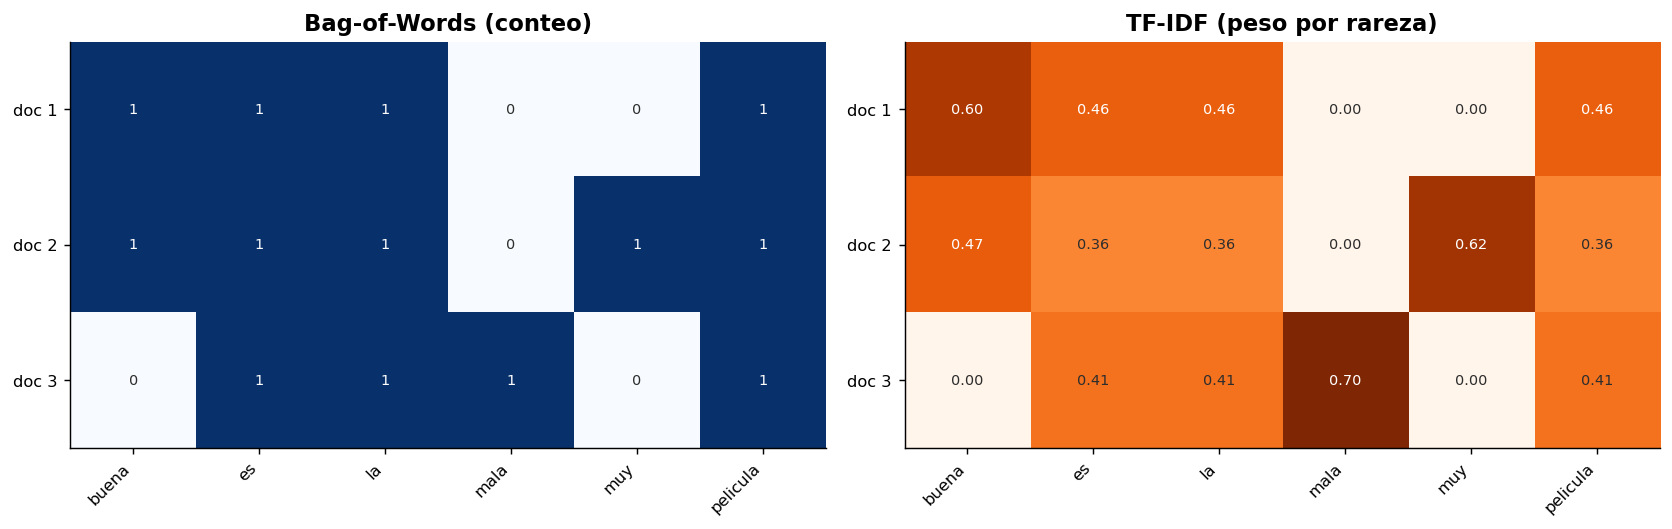
\includegraphics[width=0.9\textwidth]{fig_bow_tfidf.png}\end{center}
  \vspace{2pt}
  {\footnotesize\color{arcaDark}
  \textbf{Cómo leer el heatmap:} filas = documentos, columnas = palabras, color = peso. A la izquierda
  el conteo crudo (``la/película'' dominan); a la derecha TF-IDF apaga esas palabras comunes y
  \textbf{enciende} las que distinguen (``buena'', ``mala'').}
\end{frame}

\begin{frame}[fragile, shrink]{La herramienta: \texttt{TfidfVectorizer}}
  \begin{pyblock}
from sklearn.feature_extraction.text import TfidfVectorizer

vec = TfidfVectorizer(
    lowercase=True, strip_accents="unicode",  # normaliza
    min_df=3,            # ignora palabras en menos de 3 documentos (ruido raro)
    ngram_range=(1, 2),  # cuenta palabras Y pares de palabras ("no gusto")
    max_features=30000)  # tope de columnas

X = vec.fit_transform(textos)   # -> matriz dispersa (documentos x palabras)
  \end{pyblock}
  \vspace{2pt}
  {\footnotesize\color{arcaDark}
  En un solo paso: \textbf{tokeniza, normaliza, construye el vocabulario, cuenta y aplica TF-IDF},
  y devuelve la matriz dispersa lista para el modelo. El \texttt{ngram\_range=(1,2)} ayuda con la
  negación al guardar pares como ``no gusto''.}
\end{frame}

% ===================== BLOQUE 4 =====================
\sectionframe{Bloque 4}{El primer clasificador\\(sentimiento y spam)}

\begin{frame}[shrink]{Antes de entrenar: ¿el problema es separable?}
  \begin{center}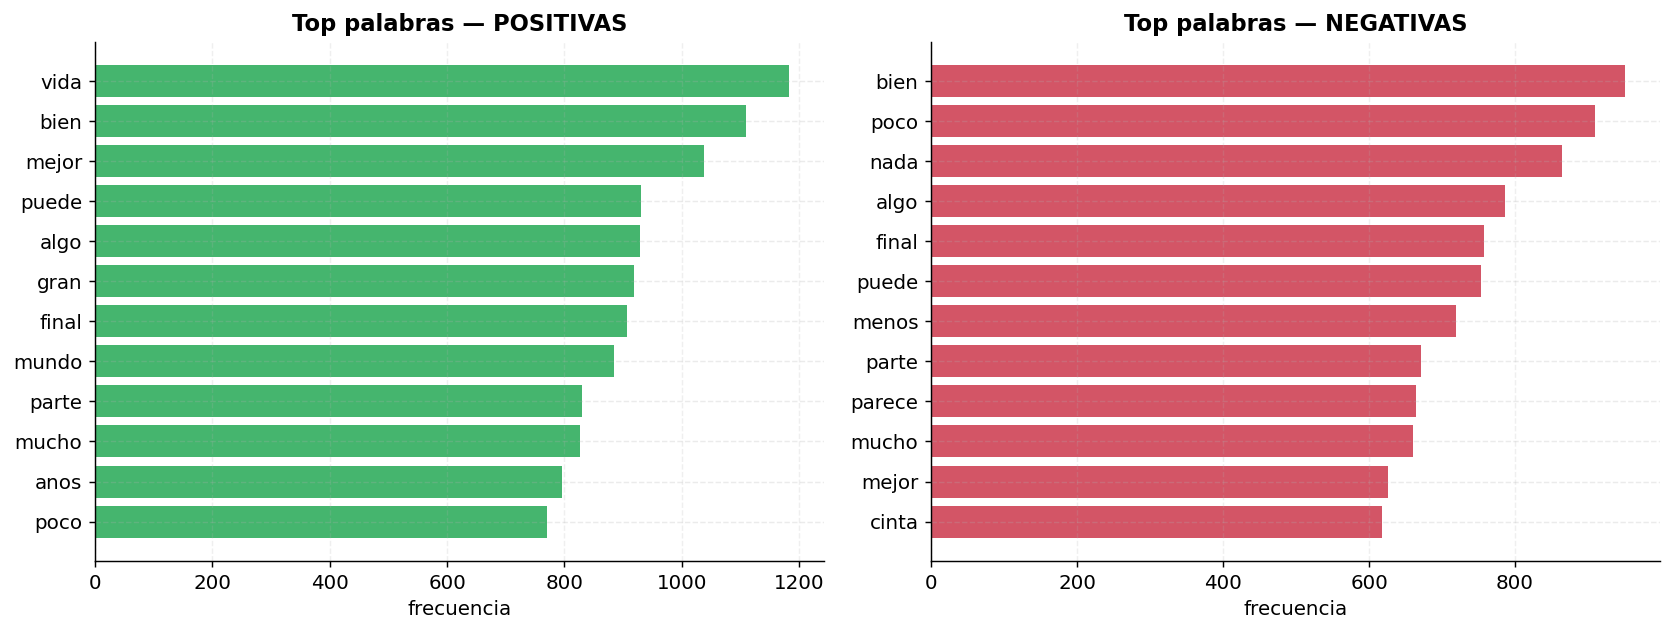
\includegraphics[width=0.97\textwidth]{fig_eda_ngramas.png}\end{center}
  \vspace{2pt}
  {\footnotesize\color{arcaDark}
  Quitando stopwords, las palabras de contenido más frecuentes ya insinúan la señal: las clases se
  distinguen \textbf{antes} de entrenar nada --- como mirar un scatter en datos tabulares.}
\end{frame}

\begin{frame}[fragile, shrink]{Sentimiento --- el mismo ML del Módulo 4}
  \begin{pyblock}
from sklearn.model_selection import train_test_split
from sklearn.linear_model import LogisticRegression

X_tr, X_te, y_tr, y_te = train_test_split(textos, etiquetas, test_size=0.2)
clf = LogisticRegression().fit(vec.fit_transform(X_tr), y_tr)   # entrena
clf.predict(vec.transform(["una obra maestra"]))                # -> positivo
  \end{pyblock}
  \vspace{2pt}
  {\footnotesize\color{arcaDark}
  No hay modelo nuevo: es la \textbf{misma Regresión Logística} que ya conoces. Lo único nuevo es
  convertir el texto en la matriz TF-IDF. Separamos en \textbf{entrenamiento / prueba} para medir
  honestamente sobre datos que el modelo no vio.}
\end{frame}

\begin{frame}[shrink]{Resultado e interpretabilidad}
  \begin{columns}[c]
    \begin{column}{0.5\textwidth}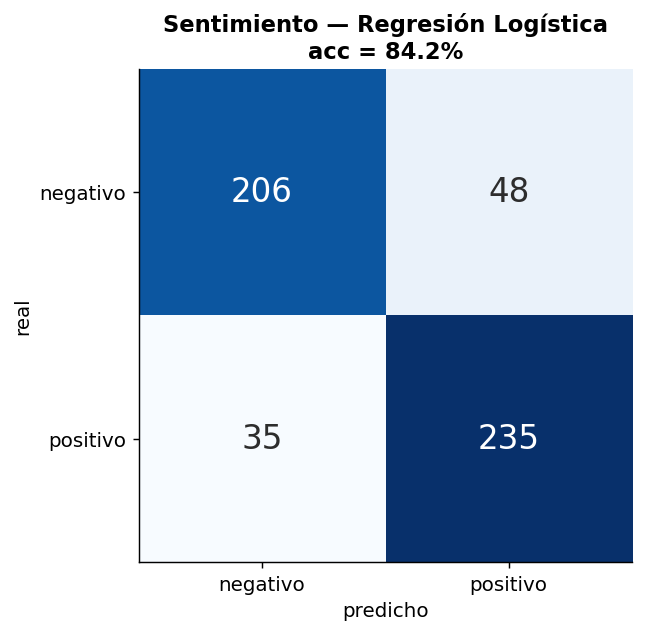
\includegraphics[width=\textwidth]{fig_sentiment_confusion.png}\end{column}
    \begin{column}{0.48\textwidth}
      {\footnotesize\color{arcaDark}
      \textbf{$\sim$84\%} de acierto en el conjunto de prueba, con un modelo que entrena en segundos.\par
      \vspace{5pt}
      Y es \textbf{interpretable}: los pesos del modelo dicen qué palabras empujan a cada clase.
      Puedes explicarle al negocio por qué decide lo que decide.}
    \end{column}
  \end{columns}
  \vspace{2pt}
  \begin{center}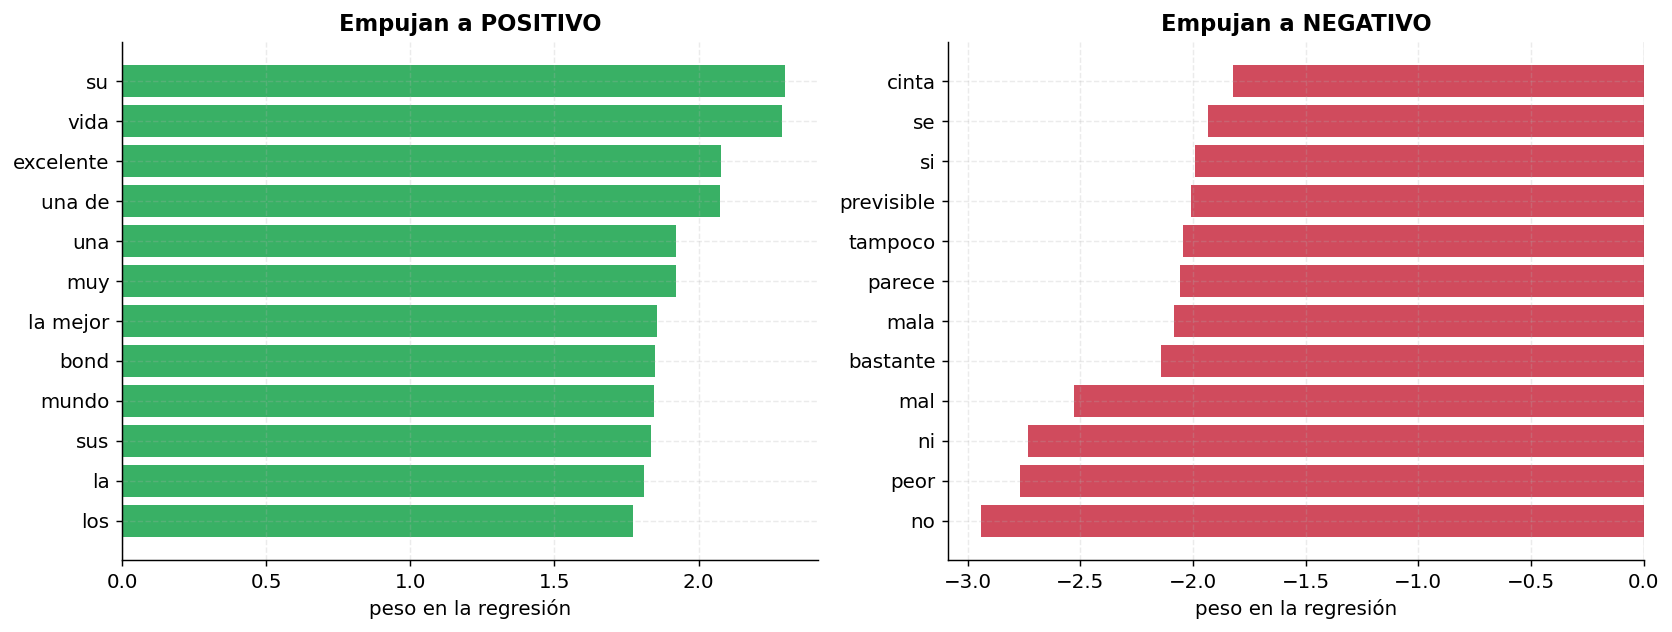
\includegraphics[width=0.84\textwidth]{fig_sentiment_coefs.png}\end{center}
\end{frame}

\begin{frame}[shrink]{Las mismas herramientas resuelven el spam}
  \begin{center}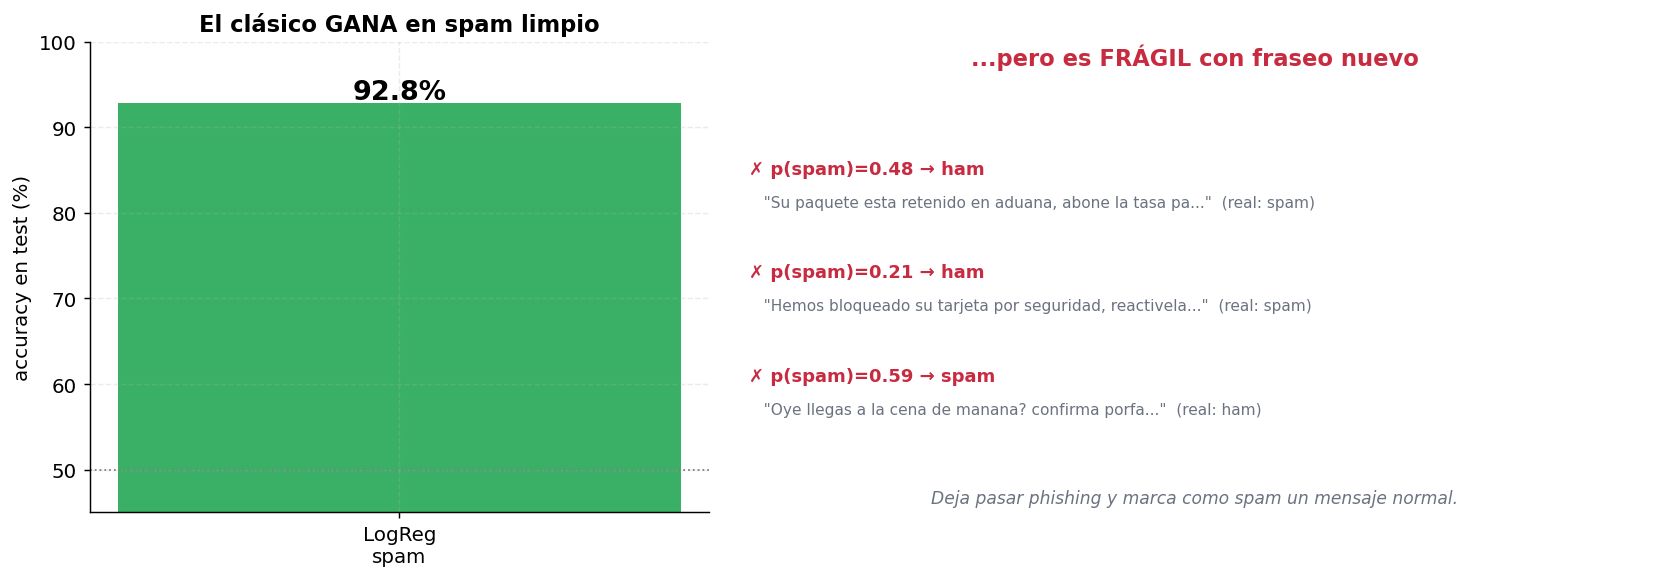
\includegraphics[width=0.96\textwidth]{fig_spam_resultado.png}\end{center}
  \vspace{2pt}
  \begin{tcolorbox}[colback=arcaGray, colframe=arcaRed, leftrule=3pt, boxrule=0pt, sharp corners, left=8pt, right=8pt, top=4pt, bottom=4pt]
    {\footnotesize\color{arcaDark}
    Cambiamos el corpus (SMS spam/ham) y \textbf{reusamos el mismo pipeline}: train/test, TF-IDF y
    Regresión Logística. Sobre los mensajes de prueba (que no vio al entrenar) acierta el
    \textbf{93\%}. \textbf{Lección:} las herramientas que aprendimos son generales y ya resuelven
    problemas reales.}
  \end{tcolorbox}
\end{frame}

% ===================== BLOQUE 5 =====================
\sectionframe{Bloque 5}{El límite de contar palabras:\\el orden y el significado}

\begin{frame}[shrink]{Problema 1: el conteo no ve el orden}
  \vspace{2pt}
  \begin{center}
  {\footnotesize\renewcommand{\arraystretch}{1.3}
  \begin{tabular}{r|ccccc}
     & \cellcolor{arcaGray}me & \cellcolor{arcaGray}gusto & \cellcolor{arcaGray}la & \cellcolor{arcaGray}película & \cellcolor{arcaGray}\textbf{no} \\\hline
    \cellcolor{codeGreen!15}``me gustó la película'' & 1 & 1 & 1 & 1 & 0 \\
    \cellcolor{arcaRed!12}``no me gustó la película'' & 1 & 1 & 1 & 1 & \cellcolor{codeOrange!35}1 \\
  \end{tabular}}
  \end{center}
  \vspace{4pt}
  {\footnotesize\color{arcaDark}
  ``me gustó la película'' (positivo) y ``no me gustó la película'' (negativo) tienen vectores
  \textbf{casi idénticos}: solo difieren en la columna ``no''. Significan lo \textbf{opuesto}, pero
  para el conteo son casi el mismo punto. \textbf{El orden y la negación se pierden.}}
\end{frame}

\begin{frame}[shrink]{Problema 2: las palabras no tienen relación entre sí}
  \vspace{2pt}
  \begin{center}
  {\footnotesize\renewcommand{\arraystretch}{1.3}
  \begin{tabular}{r|ccccc}
    \cellcolor{arcaGray}\textbf{bueno}  & \cellcolor{codeGreen!30}1 & 0 & 0 & 0 & 0 \\
    \cellcolor{arcaGray}\textbf{genial} & 0 & \cellcolor{codeGreen!30}1 & 0 & 0 & 0 \\
    \cellcolor{arcaGray}\textbf{mesa}   & 0 & 0 & \cellcolor{codeBlue!30}1 & 0 & 0 \\
  \end{tabular}}
  \end{center}
  \vspace{4pt}
  {\footnotesize\color{arcaDark}
  Cada palabra es una \textbf{columna independiente} (un ``1'' en su propia posición). Para el modelo,
  ``bueno'' está \textbf{tan lejos} de ``genial'' como de ``mesa''. \textbf{No sabe que ``bueno'' y
  ``genial'' significan casi lo mismo.}}
  \vspace{4pt}
  \begin{tcolorbox}[colback=arcaRed!8, colframe=arcaRed, leftrule=3pt, boxrule=0pt, sharp corners, left=8pt, right=8pt, top=4pt, bottom=4pt]
    {\footnotesize\color{arcaDark}\bfseries
    Por eso falla con \textbf{fraseo nuevo}: si un spam usa palabras que no vio, está perdido. Necesitamos
    que las palabras \textbf{parecidas} estén \textbf{cerca}. Eso son los embeddings.}
  \end{tcolorbox}
\end{frame}

% ===================== BLOQUE 6 =====================
\sectionframe{Bloque 6}{Del símbolo al significado:\\embeddings}

\begin{frame}[shrink]{La idea: cada palabra es un vector, el significado es geometría}
  \begin{columns}[c]
    \begin{column}{0.5\textwidth}
      \begin{center}
      \begin{tikzpicture}[scale=0.95, every node/.style={font=\scriptsize}]
        \draw[->,textMuted] (-0.2,0)--(4,0); \draw[->,textMuted] (0,-0.2)--(0,3.2);
        \fill[codeGreen] (0.7,2.5) circle (2pt) node[above]{excelente};
        \fill[codeGreen] (1.1,2.1) circle (2pt) node[right]{buena};
        \fill[codeGreen] (0.5,2.0) circle (2pt) node[left]{genial};
        \draw[codeGreen, dashed] (0.8,2.2) circle (0.85);
        \fill[arcaRed] (3.1,0.7) circle (2pt) node[above]{mala};
        \fill[arcaRed] (3.4,0.4) circle (2pt) node[right]{aburrida};
        \fill[arcaRed] (2.9,0.35) circle (2pt) node[left]{lenta};
        \draw[arcaRed, dashed] (3.15,0.5) circle (0.7);
      \end{tikzpicture}
      \end{center}
    \end{column}
    \begin{column}{0.5\textwidth}
      {\footnotesize\color{arcaDark}
      En vez de un índice arbitrario, a cada palabra le damos un \textbf{vector} de (p.ej.) 100 números.\par
      \vspace{6pt}
      Lo entrenamos para que palabras de \textbf{significado parecido} queden \textbf{cerca} en el
      espacio. El significado se vuelve \textbf{geometría}.\par
      \vspace{6pt}
      Es la misma idea del \textbf{espacio latente} del autoencoder (clase 29) y de PCA: pocas
      dimensiones que organizan el sentido.}
    \end{column}
  \end{columns}
\end{frame}

\begin{frame}[shrink]{Word2Vec --- de dónde viene}
  \begin{itemize}\setlength{\itemsep}{5pt}\footnotesize
    \item \textbf{2013, Google} --- Tomáš Mikolov y su equipo publican \textbf{Word2Vec}.
    \item Fue un hito: mostró cómo aprender un \textbf{vector por palabra} de forma eficiente a partir
      de \textbf{enormes cantidades de texto} sin etiquetar (aprendizaje auto-supervisado).
    \item Antes, las palabras eran símbolos sin relación (one-hot, como vimos). Word2Vec popularizó
      la idea de \textbf{``significado como geometría''}.
    \item Hizo famosa la ``aritmética de palabras'': \textbf{rey $-$ hombre $+$ mujer $\approx$ reina}.
  \end{itemize}
  \vspace{4pt}
  \begin{tcolorbox}[colback=arcaGray, colframe=arcaRed, leftrule=3pt, boxrule=0pt, sharp corners, left=8pt, right=8pt, top=4pt, bottom=4pt]
    {\footnotesize\color{arcaDark}
    \textbf{Qué hace, en una frase:} aprende a colocar cada palabra en un espacio de modo que las que
    aparecen en \textbf{contextos parecidos} queden \textbf{cerca}. Fue la semilla de todo lo que vino
    después (incluidos los transformers).}
  \end{tcolorbox}
\end{frame}

\begin{frame}[shrink]{¿Cómo se aprende? Por las compañías de cada palabra}
  \begin{center}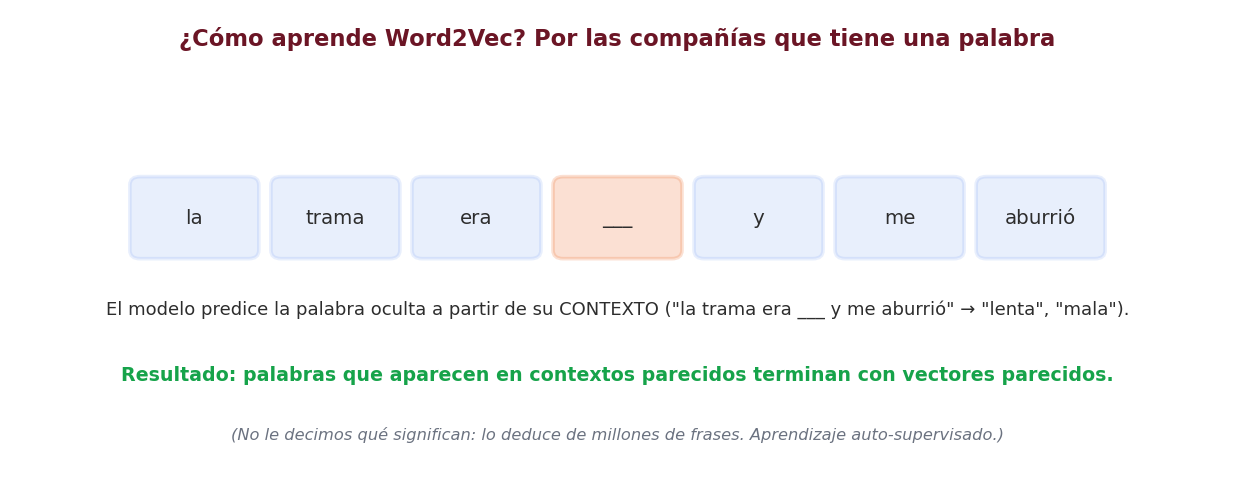
\includegraphics[width=0.95\textwidth]{fig_word2vec_idea.png}\end{center}
  \vspace{2pt}
  {\footnotesize\color{arcaDark}
  Word2Vec recorre millones de frases tapando una palabra y tratando de \textbf{adivinarla por su
  contexto} (o al revés). Para acertar, se ve obligado a darle vectores parecidos a palabras que
  comparten contexto.}
\end{frame}

\begin{frame}[fragile, shrink]{Word2Vec sobre nuestras reseñas (sin descargar nada)}
  \begin{pyblock}
from gensim.models import Word2Vec

frases = [tokenizar(t) for t in resenas]
w2v = Word2Vec(frases, vector_size=100, window=5, min_count=5, sg=1)

w2v.wv.most_similar("aburrida")
# -> [('tediosa', .72), ('boba', .70), ('monotona', .68), ...]
  \end{pyblock}
  \vspace{2pt}
  {\footnotesize\color{arcaDark}
  Sin decirle nunca qué significan, aprendió que ``aburrida'' $\approx$ ``tediosa''. \textbf{Significado
  capturado como geometría}, a partir de las palabras que la rodean.}
\end{frame}

\begin{frame}[shrink]{Vecinos por significado (reales, del corpus)}
  \begin{center}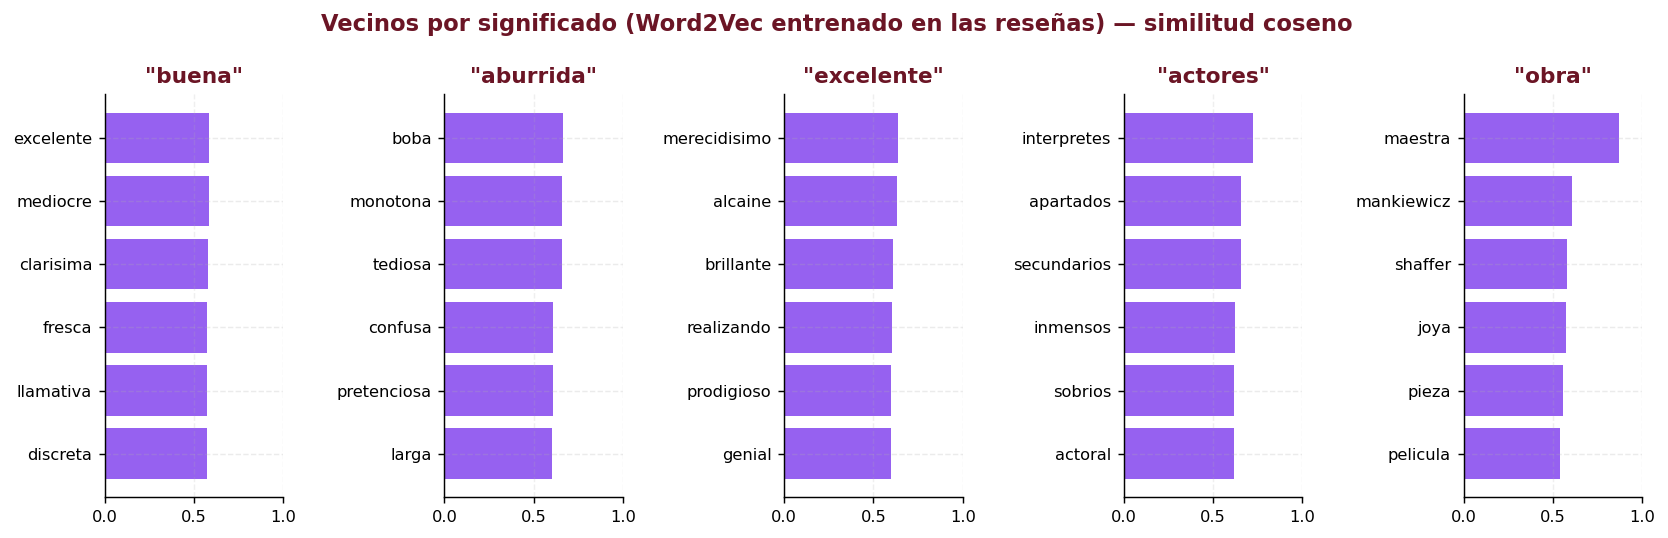
\includegraphics[width=0.98\textwidth]{fig_embeddings_vecinos.png}\end{center}
\end{frame}

\begin{frame}[shrink]{El mapa 2D de los embeddings}
  \begin{center}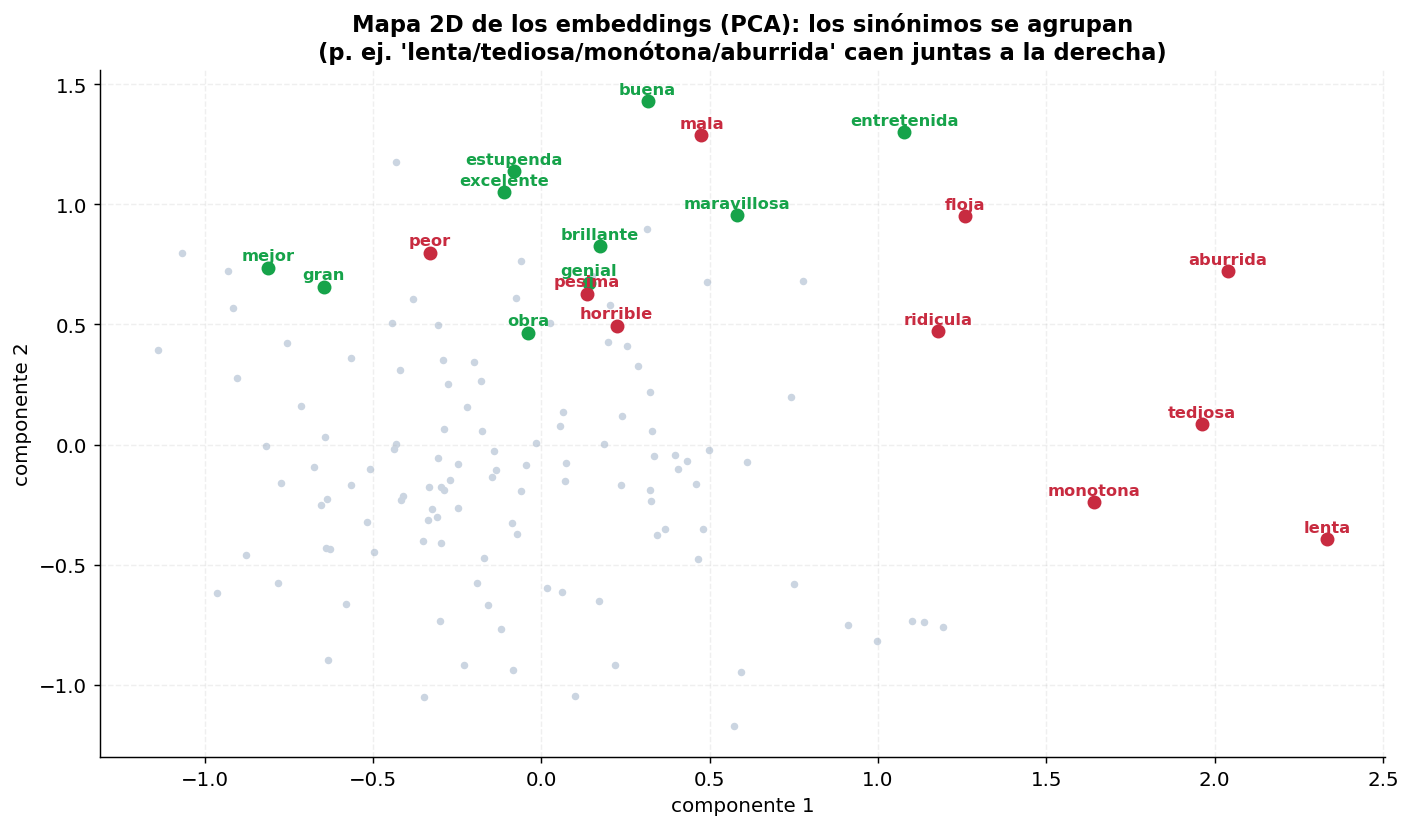
\includegraphics[width=0.78\textwidth]{fig_embeddings_2d.png}\end{center}
  \vspace{1pt}
  {\footnotesize\color{arcaDark}
  Proyección PCA (una sombra 2D de las 100 dimensiones): los sinónimos se agrupan ---
  ``lenta/tediosa/monótona/aburrida'' caen juntas a un lado.}
\end{frame}

\begin{frame}[shrink]{Comparar significados: la similitud coseno}
  \begin{columns}[c]
    \begin{column}{0.46\textwidth}
      \begin{center}
      \begin{tikzpicture}[scale=0.9, every node/.style={font=\scriptsize}]
        \draw[->,textMuted] (0,0)--(3.6,0); \draw[->,textMuted] (0,0)--(0,3.2);
        \draw[->,codeGreen, very thick] (0,0)--(2.6,1.7) node[right]{texto A};
        \draw[->,codeGreen, very thick] (0,0)--(2.9,1.2) node[right]{texto B};
        \draw[->,arcaRed, very thick] (0,0)--(0.6,2.9) node[above]{texto C};
        \draw[codeGreen] (1.0,0.65) arc (33:22:1.2);
        \node[codeGreen] at (1.5,0.45) {$\theta$ chico};
      \end{tikzpicture}
      \end{center}
    \end{column}
    \begin{column}{0.52\textwidth}
      {\footnotesize\color{arcaDark}
      La \textbf{similitud coseno} mide el \textbf{ángulo} entre dos vectores (no su longitud):\par
      \vspace{4pt}
      $\cos\theta = 1$: misma dirección $\rightarrow$ \textbf{mismo significado}.\par
      $\cos\theta = 0$: perpendiculares $\rightarrow$ \textbf{sin relación}.\par
      \vspace{4pt}
      Dos textos del mismo tema ``apuntan al mismo lado'', aunque usen palabras distintas.}
    \end{column}
  \end{columns}
\end{frame}

\begin{frame}[shrink]{Búsqueda semántica --- buscar por significado, no por palabras}
  \begin{center}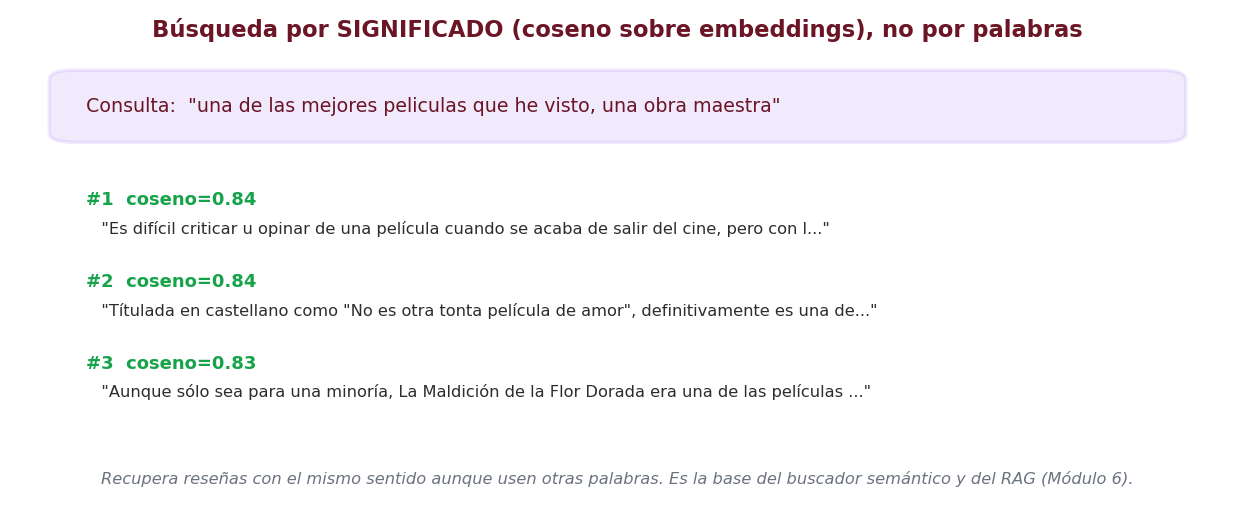
\includegraphics[width=0.95\textwidth]{fig_busqueda_coseno.png}\end{center}
  \vspace{2pt}
  \begin{tcolorbox}[colback=arcaGray, colframe=arcaRed, leftrule=3pt, boxrule=0pt, sharp corners, left=8pt, right=8pt, top=4pt, bottom=4pt]
    {\footnotesize\color{arcaDark}
    Representamos cada documento como el \textbf{promedio} de los vectores de sus palabras y buscamos
    por coseno. Aplicación de negocio: ``encuentra quejas parecidas a esta''. Es la base del buscador
    semántico y del RAG (Módulo 6).}
  \end{tcolorbox}
\end{frame}

\begin{frame}[shrink]{Lo que los embeddings todavía no resuelven}
  \begin{tcolorbox}[colback=arcaRed!8, colframe=arcaRed, leftrule=3pt, boxrule=0pt, sharp corners, left=8pt, right=8pt, top=5pt, bottom=5pt]
    {\small\color{arcaDark}
    Word2Vec le da a cada palabra \textbf{un solo} vector, fijo. Pero ``banco'' (de sentarse) y
    ``banco'' (de dinero) comparten vector. Y si promediamos ``no me gustó'', volvemos a hacer una
    bolsa: \textbf{no capturamos que ``no'' modifica a ``gustó''}.}
  \end{tcolorbox}
  \vspace{6pt}
  {\footnotesize\color{arcaDark}
  Necesitamos que el vector de una palabra \textbf{dependa de su contexto} en la frase. Eso es la
  \textbf{atención}.}
\end{frame}

% ===================== BLOQUE 7 =====================
\sectionframe{Bloque 7}{Del significado al contexto:\\atención y transformers}

\begin{frame}[shrink]{Qué es la atención}
  \begin{center}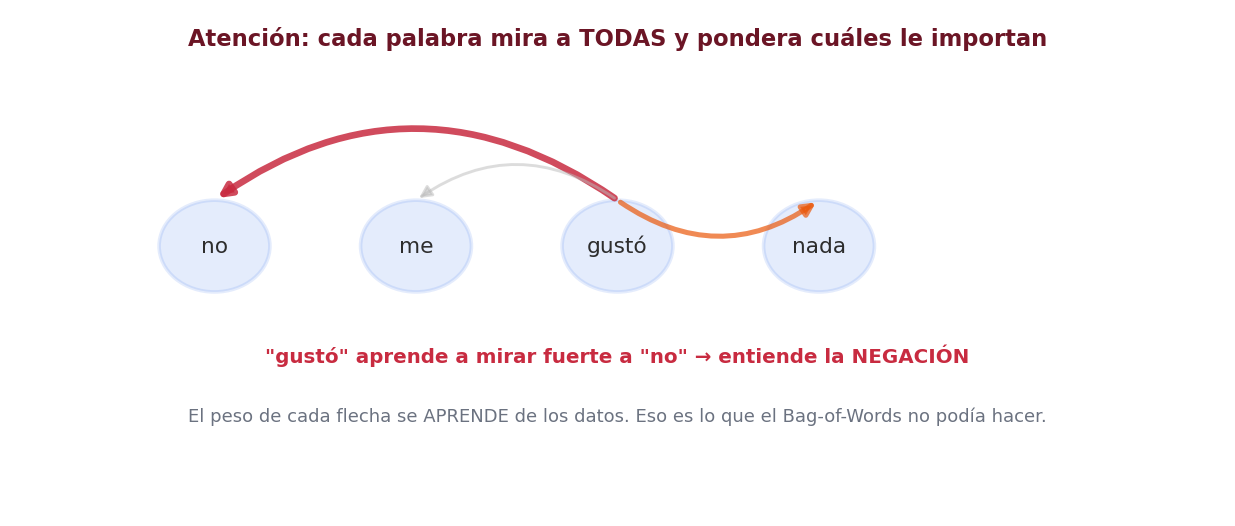
\includegraphics[width=0.95\textwidth]{fig_atencion_concepto.png}\end{center}
  \vspace{2pt}
  {\footnotesize\color{arcaDark}
  Para cada palabra, el modelo mira a \textbf{todas} las demás y aprende \textbf{cuánto pesa} cada
  una. Así ``gustó'' se relaciona con ``no'' --- lo que el conteo y los embeddings fijos no podían.}
\end{frame}

\begin{frame}[shrink]{Por dentro: Query, Key, Value}
  \begin{center}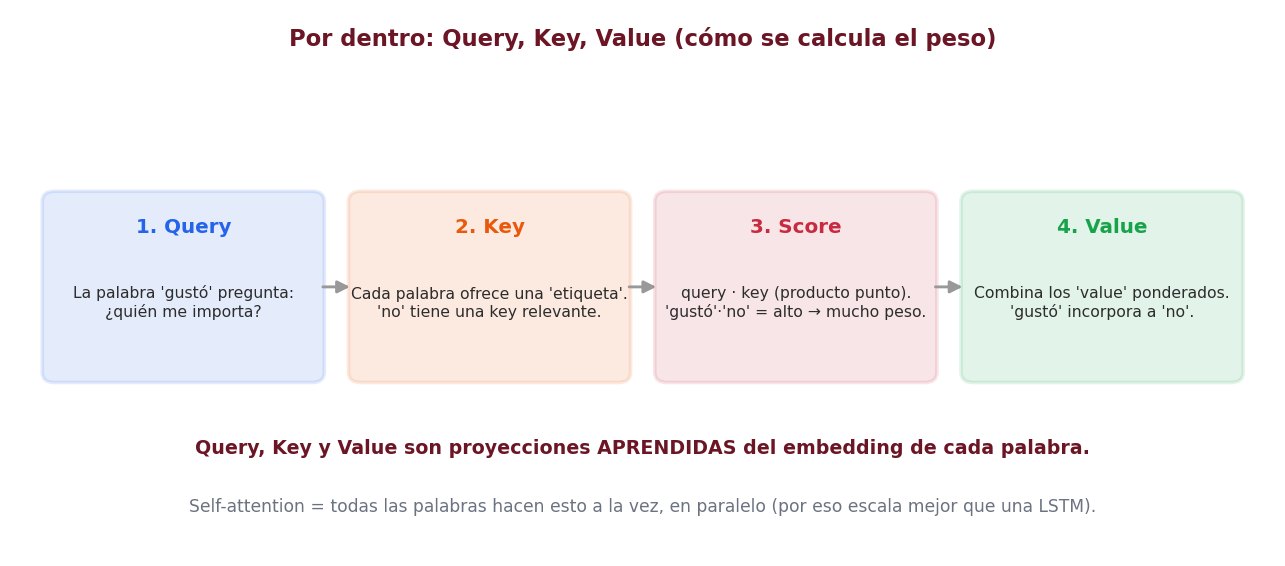
\includegraphics[width=0.97\textwidth]{fig_qkv.png}\end{center}
\end{frame}

\begin{frame}[shrink]{Un Transformer = embeddings + atención apilada}
  \begin{center}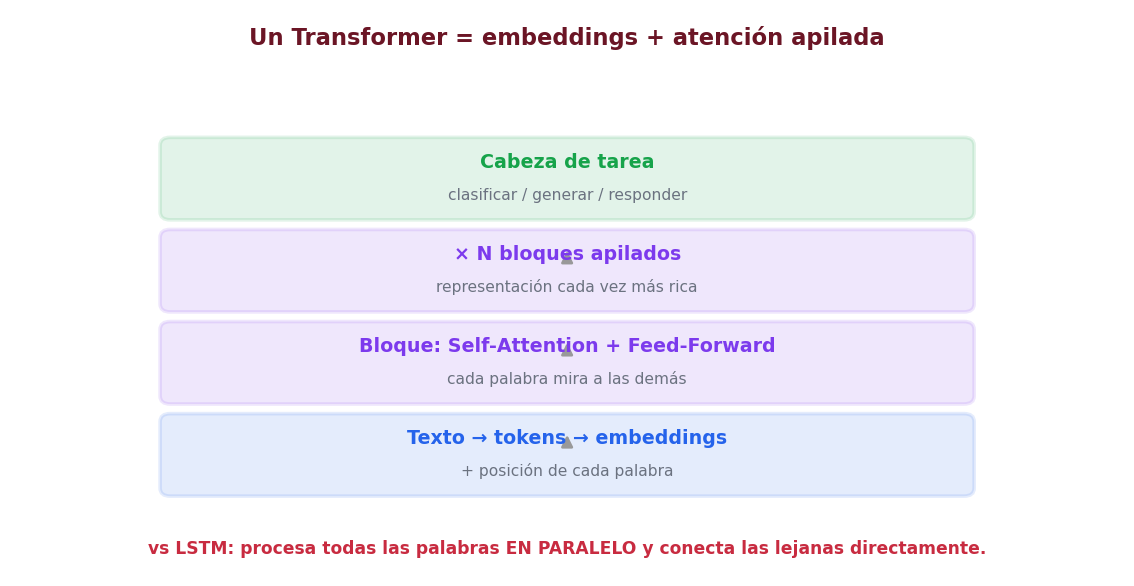
\includegraphics[width=0.8\textwidth]{fig_transformer_arquitectura.png}\end{center}
  \vspace{1pt}
  {\footnotesize\color{arcaDark}
  Apila muchos bloques de atención. Procesa todas las palabras en paralelo y conecta las lejanas
  directamente $\rightarrow$ por eso supera a la LSTM y escala a textos largos.}
\end{frame}

\begin{frame}[shrink]{\textit{Attention Is All You Need} (2017)}
  \begin{center}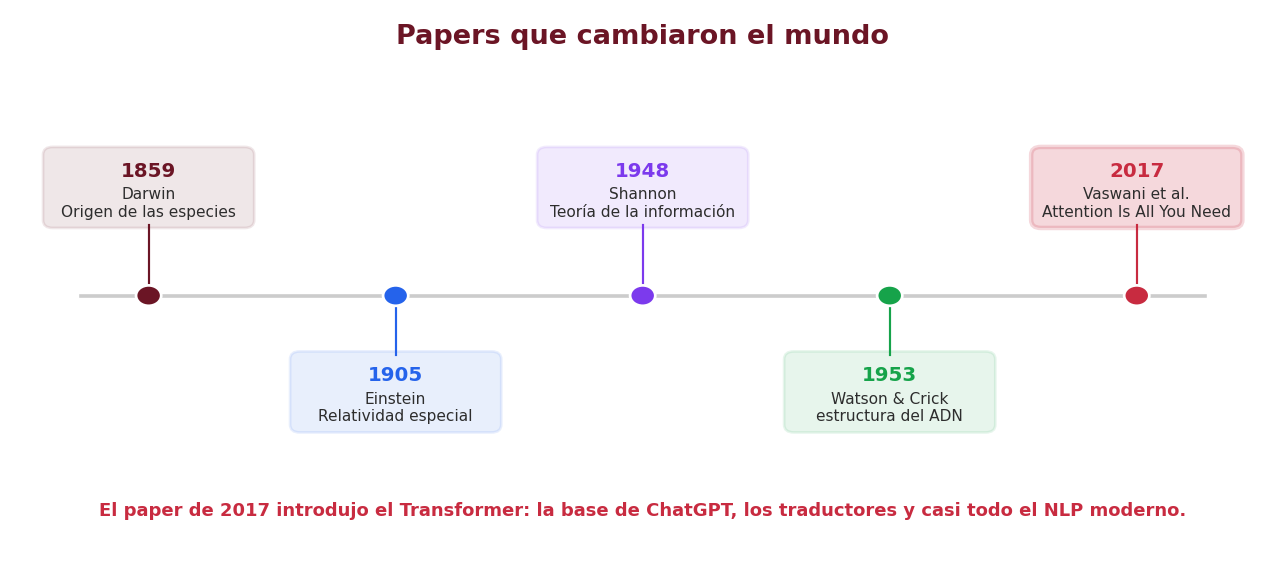
\includegraphics[width=0.97\textwidth]{fig_papers_historia.png}\end{center}
\end{frame}

\begin{frame}[fragile, shrink]{Un mini-modelo de atención en Keras}
  \begin{pyblock}
from tensorflow.keras import layers, models

inp = layers.Input(shape=(MAXLEN,))
emb = layers.Embedding(VOCAB, DIM)(inp)
att = layers.MultiHeadAttention(num_heads=1, key_dim=DIM)
ctx, scores = att(emb, emb, return_attention_scores=True)  # la atencion
x = layers.GlobalAveragePooling1D()(ctx)
out = layers.Dense(1, activation="sigmoid")(layers.Dense(32, "relu")(x))
modelo = models.Model(inp, out)
  \end{pyblock}
  \vspace{2pt}
  {\footnotesize\color{arcaDark}
  Keras puro (corre en Colab, nada que descargar). Guardamos \texttt{scores} para \textbf{ver a dónde
  mira} cada palabra.}
\end{frame}

\begin{frame}[shrink]{Visualizar la atención}
  \begin{columns}[c]
    \begin{column}{0.5\textwidth}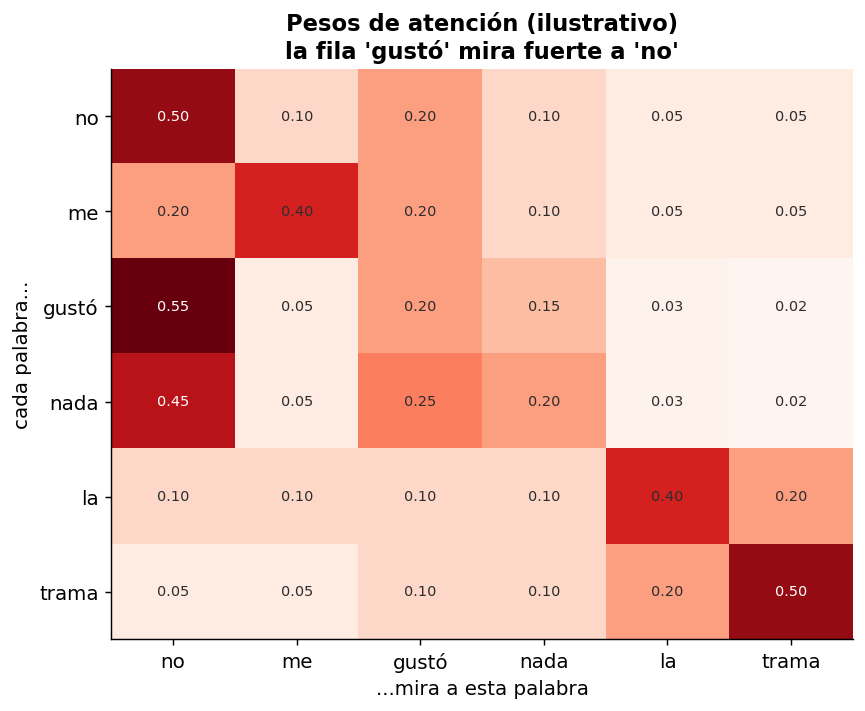
\includegraphics[width=\textwidth]{fig_atencion_heatmap.png}\end{column}
    \begin{column}{0.48\textwidth}
      {\footnotesize\color{arcaDark}
      Cada fila = una palabra; las columnas = a quién mira. El modelo \textbf{puede} relacionar
      ``gustó'' con ``no''.\par\vspace{5pt}
      \textbf{No esperes que le gane al baseline aquí:} con 2.600 reseñas no brilla. Su poder real
      aparece con \textbf{pre-entrenamiento a escala}.}
    \end{column}
  \end{columns}
  \vspace{2pt}
  {\scriptsize\color{textMuted}(Mapa ilustrativo; el real se genera en vivo en el notebook.)}
\end{frame}

\begin{frame}[shrink]{El límite --- y por qué usamos modelos pre-entrenados}
  \begin{center}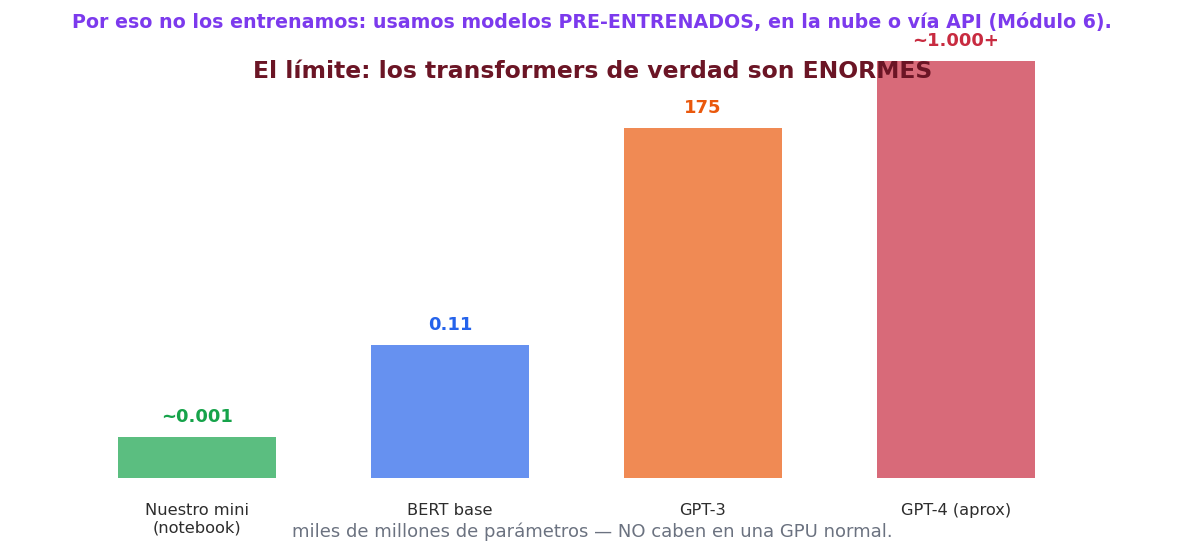
\includegraphics[width=0.93\textwidth]{fig_transformer_limite.png}\end{center}
\end{frame}

% ===================== CIERRE =====================
\sectionframe{Cierre}{Lo que te llevas}

\begin{frame}[shrink]{Las 4 representaciones, lado a lado}
  \vspace{10pt}
  {\small
  \begin{tabular}{@{}p{2.6cm}p{3.8cm}p{3.1cm}p{3.2cm}@{}}
    \toprule
    \textbf{Técnica} & \textbf{Qué captura} & \textbf{Falla en} & \textbf{Cuándo usarla}\\
    \midrule
    \textcolor{codeBlue}{\textbf{Bag-of-Words}} & qué palabras hay & el orden, la rareza & línea base rápida\\[3pt]
    \textcolor{codeOrange}{\textbf{TF-IDF}} & cuáles importan & el significado & clasificar e interpretar\\[3pt]
    \textcolor{codeGreen}{\textbf{Embeddings}} & sinónimos cercanos & el contexto (vector fijo) & buscar por significado\\[3pt]
    \textcolor{codePurple}{\textbf{Atención}} & significado en contexto & necesita escala (pre-entrenar) & contexto complejo / generar\\
    \bottomrule
  \end{tabular}}
  \vspace{10pt}
  \begin{tcolorbox}[colback=arcaRed!8, colframe=arcaRed, leftrule=3pt, boxrule=0pt, sharp corners, left=8pt, right=8pt, top=4pt, bottom=4pt]
    {\footnotesize\color{arcaDark}\bfseries
    Empieza simple. Sube de complejidad solo cuando lo simple ya no alcanza.}
  \end{tcolorbox}
\end{frame}

\begin{frame}[shrink]{Árbol de decisión práctico}
  \begin{center}
\includegraphics[width=0.95\textwidth]{fig_decision_tree.png}\end{center}
\end{frame}

\begin{frame}[shrink]{Lo que te llevas hoy}
  \begin{enumerate}\setlength{\itemsep}{3pt}\footnotesize
    \item NLP es, ante todo, \textbf{convertir texto en números} que capturan cada vez más significado.
    \item \textbf{Bag-of-Words / TF-IDF}: simples, rápidos, interpretables. Resuelven sentimiento ($\sim$84\%) y spam ($\sim$93\%).
    \item \textbf{Zipf} explica las stopwords, TF-IDF y la matriz dispersa.
    \item \textbf{Embeddings}: el significado como geometría; \textbf{búsqueda coseno} = buscar por sentido.
    \item \textbf{Atención}: el significado depende del contexto; base de los \textbf{Transformers} y los LLMs.
    \item \textbf{Empieza simple.} Sube de complejidad solo cuando lo simple ya no alcanza.
  \end{enumerate}
  \vspace{4pt}
  {\footnotesize\color{arcaDark}\bfseries Clase 34: transformers y modelos pre-entrenados en acción (rampa al Módulo 6).}
\end{frame}

\sectionframe{Gracias}{Clase 33 --- Introducción a NLP\\github.com/cmosquerat/arca-diplomado}

\end{document}
